%\vspace{-0.12in}
\chapter{Evaluations}
\label{sec:eval}
%The implementation of \sys was implicitly described in prior sections.
%(most modules
%were implemented in Java).
Our experiments (model checking) are performed on a MacBook Pro with macOS Sierra, 2.9 GHz Intel Core i5, 16 GB 1867 MHz DDR3, and 256 GB SSD.
We check if there are violations of the properties 
discussed in \S\ref{sec:model}.
%Table~\ref{table:racescenarios}
We also look at other performance metrics such as the running times,
and the scale ratio (which quantifies the reduction in the number of event handlers
to be jointly verified) to evaluate \sys.

%\vspace{-0.17in}
\section{Test Cases and Configurations}
We perform four different sets of experiments described below.
The first three examine the fidelity with which bad apps and configurations are identified.
The last set evaluates the performance of different design choices we make.

{\bf Market apps with expert configurations:}
We check the safety properties with
150 apps (assuming they are benign) from the {\color{black}SmartThings' market place \cite{SmartThingsGitHub,STCommunitySmartApps,Samsung:smartthingsmanage}.}
We (the authors) came up with independent
configurations for the apps (based on common sense with regards to how the apps may be used).
To illustrate, consider the app \textsl{Virtual Thermostat}, the required input to which is shown in Figure~\ref{inputexample}.
Assume that the following devices are deployed:
(1) one temperature sensor (myTempMeas), (2) one outlet to control the heater (myHeaterOutlet),
(3) one outlet to control the air conditioner (myACOutlet),
(4) one outlet to control the light in the living room (livRoomBulbOutlet),
(5) one outlet to control the light in the bedroom (bedRoomBulbOutlet),
(6) one outlet to control the light in the bathroom (batRoomBulbOutlet),
(7) one motion sensor in the living room (livRoomMotion),
and (8) one motion sensor in the bathroom (batRoomMotion).
Our configuration is as follows:
myTempMeas for the temperature sensor (line 3 in Figure~\ref{inputexample}),
myACOutlet for ``outlets" (line 7 in Figure~\ref{inputexample}),
$75$ as the ``{\color{black} setpoint}" temperature if people are present (line 9 in Figure~\ref{inputexample}),
livRoomMotion for ``motion" (line 12 in Figure \ref{inputexample}),
$10$ ``minutes" for turning off the AC/heater when no motion is sensed (line 15 in Figure~\ref{inputexample}),
%\krish{Say what this does as in prior cases},
$85$ as the ``emergencySetPoint" temperature at which the AC is turned on (to set) regardless of
whether people are present (line 18 in Figure \ref{inputexample}),
and ``cool" for ``mode" (line 21 in Figure \ref{inputexample}).
%\krish{Unless something isn't obvious above no need for this. But provide some description as the ones I did}
%We think that this configuration is reasonable because those of both air conditioner and heater, (2) ``cool" instead of ``heat" should go with air conditioner, and (3) other remaining fields are quite straightforward.

We randomly divide the 150 apps into six groups (25 apps per group) with one configuration each,
and feed them into \sys.
Upon encountering a violation, we remove the minimum number of the associated apps (\textit{e.g.}, if there are two apps causing conflicting commands, we randomly remove one of them);
%\krish{what are conflicting commands ? Hopefully this has been described earlier.}\thomas{Yes, it is}
we then iterate the process. The experiment stops when no violation is detected.
These experiments are performed with and without device/communication failures.

\hfill \break

{\bf Market apps with non-expert configurations:}
To eliminate biases, we also conduct a user study where we request 7 independent student volunteers
to configure 10 groups of apps with the assumption that they would deploy them at home.
Each group comprises of about 5 related apps (as determined by our app dependency analyzer).
A group receives one configuration from each volunteer and this leads to a total of 70 configurations.
Our Office of Research Integrity determined that
there was no need to go through an IRB approval process (since no private information is collected).

{\bf Malicious apps:}
We consider 25 malicious apps created in~\cite{Jia:contexiot}.
In this set, we find that only 9 apps are relevant
to our evaluations (\textit{e.g.}, affect the physical state and can be compiled correctly by the SmartThings' own web-based IDE).
%\textcolor{black}{among 25 apps, since there are several duplicates, we have 20 apps after removing the duplicates; moreover, four apps (\textit{i.e.}, \textit{BackDoorPincodeInjection}, \textit{LockAccessRevocation}, \textit{LockManager}, and \textit{MaliciousCameraIPC}) get compile errors with Samsung SmartThings' web-based IDE (16 apps remaining); we manually analyzed the source code of the app \textit{Disabling Vacation Mode} and did not find any malicious behaviors (15 apps remaining); attacking techniques done by the two apps \textit{CO Detector} and \textit{Hello Home} are out of our problem scope because they just add some extra content to an SMS message (13 apps remaining);
There are four apps that \sys cannot currently handle viz., \textit{Midnight Camera}, \textit{Auto Camera}, \textit{Auto Camera 2}, and \textit{Alarm Manager}, since they dynamically discover and control the devices in the system; we will extend \sys to handle such apps in future work.
%however, their malicious functions can be detected by \sys; for example, the three apps (\textit{Auto Camera}, \textit{Auto Camera 2}, and \textit{Alarm Manager}) would violate information leakage property when the command \textit{httpPost} is executed, and the app \textit{Midnight Camera} would violate the property \textit{A specific light close to surveillance camera is turned off at night}. \zhiyun{I don't understand why we can detect problems with three of these apps even when we admit \sys cannot handle them.}\thomas{These apps cannot be modeled and verified by \sys. If we remove the ``dynamic discovery" code, these apps can be verified by \sys and their adversary techniques can be detected by \sys using the properties we have defined.}
%\thomas{Do we need to explain why other apps are not relevant here?} . \krish{Yes -- this is where you would discuss that.}
We evaluate whether \sys correctly attributes these malicious apps when they are installed together with other apps.
The configurations of the 9 malicious apps are identical to those
in \cite{Jia:contexiot}. We also choose 11 potentially bad apps (found via the previous experiments) from the market place 
for a total of 20 bad apps. In conjunction, we select 10 good apps from the market place to create a reasonable input set. Here, we specifically evaluate the fidelity of our attribution module. %with the input data set and the stable system.

\begin{table*}[tb]
\scriptsize
\caption{Verification results with market apps.}
%\vspace{-0.12in}
\label{market_apps}
\centering
%\bf
{\begin{tabular}{| p{2.2cm} | p{1.4cm} | p{4.5cm} | p{4.5cm} |}
\hline
{\bf Violation type} & {\bf Number of violations} & {\bf Example violated property} & {\bf Apps related to example}\\
\hline
Conflicting commands & 8 & A light receives ``on" and ``off" simultaneously & (Brighten Dark Places, Let There Be Dark)\\
%\hline
%2 & A configured outlet is turned off when someone is still at home & 1 & (Curling Iron)\\
\hline
Repeated commands & 10 & A light receives repeated ``on'' commands & (Automated light, Brighten My Path)\\
\hline
\multirow{2}{2.2cm}{Unsafe physical states} & \multirow{2}{*}{20} & A heater is turned off at night when temperature is below a predefined threshold & (Energy Saver)\\ \cline{3-4}
 & & The main door is unlocked when people are sleeping at night & (Light Follows Me, Light Off When Close, GoodNight, Unlock Door)\\ \cline{3-4}
\hline
\end{tabular}}
%\vspace{-0.12in}
\end{table*}

\begin{table}[tb]
\ssp
\scriptsize
\caption{Verification result with market apps, with volunteer configuration.}
%\zhiyun{violation ratio in this table and the violation ratio in the next table are both called the same thing but they are actually trying to capture different things. I think we should call it something else. Maybe ``Percentage of bad configurations''?} \thomas{I have modified the term.}
\label{user_market_apps}
\centering
{
\begin{tabular}{| c | p{5.5cm} | p{4.5cm} | p{2.0cm} |}
\hline
{\bf Group} & {\bf Violations} & {\bf Related Apps} & {\bf Percentage of bad configs}\\
\hline
\multirow{12}{*}{1}  & A microwave is turned on when no one is at home & Big Turn On, Auto Mode Change & 28.6\%\\ \cline{2-4}
	& \multirow{2}{5.5cm}{An AC and a heater are both turned on} & Big Turn On, Auto Mode Change & 28.6\%\\ \cline{3-4}
	&	& The Big Switch & 42.9\%\\ \cline{2-4}
	& \multirow{4}{5.5cm}{A heater is turned on when temperature is above a predefined threshold and no one is at home} & Big Turn On, Auto Mode Change & 28.6\%\\ \cline{3-4}
	&	& The Big Switch & 42.9\% \\[3ex] \cline{2-4}
	& \multirow{3}{5.5cm}{An AC is turned on when temperature is below a predefined threshold} & Big Turn On, Auto Mode Change & 42.9\%\\ \cline{3-4}
	&	& The Big Switch & 71.4\%\\
\hline
\multirow{13}{*}{2}  &  \multirow{9}{7cm}{Conflicting commands}  & Brighten Dark Places, Let There Be Dark! & 85.7\%\\ \cline{3-4}
	&	& Once a Day, Let There Be Dark! & 14.3\%\\ \cline{3-4}
	&	& Once a Day, Curling Iron & 71.4\%\\ \cline{3-4}
	&	& Once a Day, Light On Motion & 28.6\%\\ \cline{3-4}
	&	& Brighten Dark Places, Once a Day & 14.3\%\\ \cline{2-4}
	& \multirow{4}{5.5cm}{Repeated commands} & Curling Iron, Light On Motion & 42.9\%\\ \cline{3-4}
	&	& Once a Day, Let There Be Dark! & 14.3\%\\ \cline{2-4}
	& An AC and a heater are both turned on & Once a Day & 28.6\%\\ \cline{2-4}
	%&	& Light on Motion & 14.3\%\\ \cline{2-4}
	& A heater is turned on when temperature is above a predefined threshold & Once a Day & 28.6\%\\ \cline{2-4}
	%&	& Light on Motion & 14.3\%\\ \cline{2-4}
	& An AC is turned on when temperature is below a predefined threshold & Once a Day & 57.1\%\\ \cline{2-4}
	%&	& Light on Motion & 14.3\%\\
\hline
3 & No violation & & \\
\hline
\end{tabular}
}
\end{table}

\begin{table}[tb]
\ssp
\scriptsize
\caption{Verification result with market apps, with volunteer configuration (continue).}
%\zhiyun{violation ratio in this table and the violation ratio in the next table are both called the same thing but they are actually trying to capture different things. I think we should call it something else. Maybe ``Percentage of bad configurations''?} \thomas{I have modified the term.}
\label{user_market_apps1}
\centering
{
\begin{tabular}{| c | p{5.5cm} | p{4.5cm} | p{2.0cm} |}
\hline
{\bf Group} & {\bf Violations} & {\bf Related Apps} & {\bf Percentage of bad configs}\\
\hline
\multirow{9}{*}{4}  & An AC is turned off when temperature is above a predefined threshold & Energy Saver & 42.9\%\\ \cline{2-4}
	& 	A heater is turned off when temperature is below a predefined threshold & Energy Saver & 42.9\%\\ \cline{2-4}
	& \multirow{3}{5.5cm}{Repeated commands} & AND Switch, Away Mode With Eco Turn Off & 14.3\%\\ \cline{3-4}
	&	& AND Switch, Energy Saver & 14.3\%\\
\hline
5 & No violation & & \\
\hline
\multirow{8}{*}{6}  & \multirow{6}{5.5cm}{Repeated commands} & Automated light, Brighten My Path & 42.9\%\\ \cline{3-4}
	& 	& Automated light, Garage check open/close App & 14.3\%\\ \cline{3-4}
	& 	& Brighten My Path, Garage check open/close App & 14.3\%\\ \cline{2-4}
	%& An AC and a heater are both turned on & Brighten My Path & 28.6\%\\ \cline{2-4}
	%& An AC is turned on when temperature is below a predefined threshold & Brighten My Path & 28.6\%\\ \cline{2-4}
	& An AC is turned off when temperature is above a predefined threshold at night & Light Follows Me, Light Off When Close, Big Turn Off, Good Night & 14.3\%\\ \cline{2-4}
	%& A heater is turned on when temperature is above a predefined threshold & Brighten My Path & 28.6\%\\ \cline{2-4}
	& A heater is turned off when temperature is below a predefined threshold at night & Light Follows Me, Light Off When Close, Big Turn Off, Good Night & 14.3\%\\
\hline
7 & No violation & & \\
\hline
\multirow{4}{*}{8}  & Conflicting commands & Multi-way On/Off Toggle Switch Using a Modded PEQ Door Open/Close Sensor, Undead early warning & 57.1\%\\ \cline{2-4}
	& An AC and a heater are both turned on & Virtual Thermostat & 71.4\%\\ \cline{2-4}
	& An AC is turned on when temperature is below a predefined threshold & Virtual Thermostat & 42.9\%\\ \cline{2-4}
	& A heater is turned on when temperature is above a predefined threshold & Virtual Thermostat & 28.6\%\\
\hline
9 & No violation & & \\
\hline
10 & Repeated commands & Let There Be Light!, Delayed Command Execution & 28.6\%\\
\hline
\end{tabular}
}
\end{table}


\begin{comment}
{
{\em Fourth set of experiments:}
We evaluate the verification time against number of generated events with \sys. We use the apps in a specific group of apps which did not have any violations, from the user study.
%The group comprises of five apps and all of them belong to the same dependent set (\textit{i.e.}, the apps should be verified jointly).
Table \ref{verificationtimesetup} describes the devices used by the apps. We quantize the humidity measurement outputs to five values (\textit{i.e.}, 10\%, 30\%, 50\%, 70\%, and 100\% ) and the temperature measurement outputs to three values (\textit{i.e.}, 1, 2, and 3).
\begin{table}[!h]
\scriptsize
\caption{Experiment setup to evaluate verification time.}
\label{verificationtimesetup}
\centering
\begin{tabular}{| l | c | c |}
\hline
Device type & \# of devices & \# of states/device\\
\hline
Presence sensor & 3 & 2\\
\hline
Contact sensor & 1 & 2\\
\hline
Humidity measurement sensor & 1 & 5\\
\hline
Temperature measurement sensor & 1 & 3\\
\hline
Switch & 2 & 2\\
\hline
Lock & 2 & 2\\
\hline
\end{tabular}
\end{table}
}
\end{comment}

\textcolor{black}{{\bf Performance:}
We compare the performance of concurrent \textit{versus} sequential design.
We use two bad groups of apps viz., (Auto Mode Change, Unlock Door) and (Brighten Dark Places, Let There Be Dark),
and one good group of apps viz., (Good Night, It's Too Cold) that control 3 switch devices,
3 motion sensors, and 1 temperature measurement sensor.}

%\vspace{-0.1in}
\section{Identifying Unsafe Configurations}
%\section{ContexIoT's malicious apps}
%Among 25 malicious apps, since there are several duplicates, we have 20 apps after removing the duplicate ones. Moreover, four apps (\textit{i.e.}, \textit{BackDoorPincodeInjection}, \textit{LockAccessRevocation}, \textit{LockManager}, and \textit{MaliciousCameraIPC}) got compile errors with Samsung SmartThings' web-based IDE. Therefore, there are only 16 apps remaining. We manually configured the setting for each app and verified them independently. \sys can detect the malicious behaviors of nine apps, which violated information leakage, unsafe scenario, and using security-sensitive commands properties. The $10^{th}$ app \textit{Disabling Vacation Mode} did not violate any properties (We manually analyzed the source code of this app and did not find any malicious behaviors). Attacking techniques done by the two apps \textit{CO Detector} and \textit{Hello Home} are out of our problem scope because they just added some extra content to an SMS message. \sys cannot handle the remaining four apps (\textit{i.e.}, \textit{Midnight Camera}, \textit{Auto Camera}, \textit{Auto Camera 2}, and \textit{Alarm Manager}) since they dynamically discover and subscribe to the devices in the system. However, their malicious functions can be detected by our tool. For example, the three apps (\textit{Auto Camera}, \textit{Auto Camera 2}, and \textit{Alarm Manager}) would violate information leakage property when the command \textit{httpPost} is executed, and the app \textit{Midnight Camera} would violate the property \textit{A specific light close to surveillance camera is turned off at night}.

\begin{figure}[tb]
	\ssp
    \centering
    \begin{subfigure}[t]{3.4in}
        \centering
        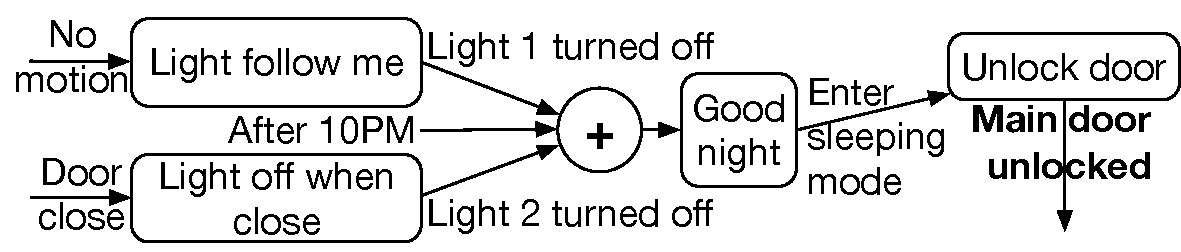
\includegraphics[width=3.4in]{violation_example}
				%\vspace{-0.06in}
		\caption{Example violation due to bad app interactions.}
        \label{violation_example}
    \end{subfigure}\\
    \vspace{0.03in}
    \begin{subfigure}[t]{3.6in}
        \centering
        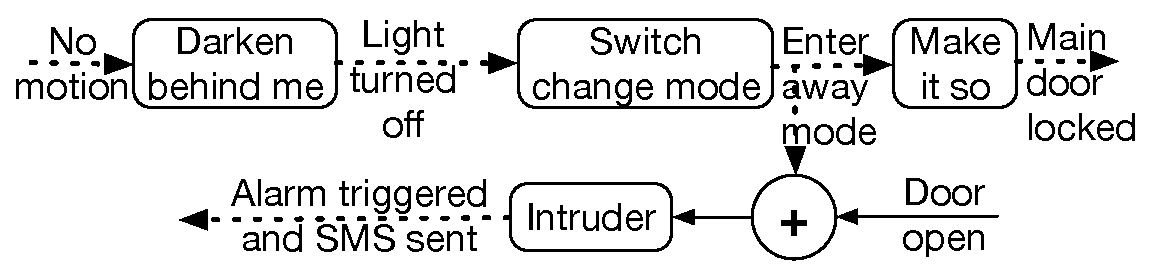
\includegraphics[width=3.6in]{device_failure}
				%\vspace{-0.06in}
        \caption{Example violation due to a device failure. Dotted arrows are
expected events that do not occur due to the failure of the motion sensor.}
		%\vspace{-0.1in}
        \label{device_failure}
    \end{subfigure}
    \caption{Violation examples: boxes depict apps and high level abstractions are
shown for inputs/outputs.}
    \label{violationexamples}
%\vspace{-0.30in}
\end{figure}

\begin{table*}[!tb]
\scriptsize
\ssp
\caption{Verification result of ContexIoT's malicious apps.}
\label{ContexIoT_apps}
\centering
{
\begin{tabular}{| c | p{1.8cm} | p{6.5cm} | p{3.9cm} |}
\hline
{\bf No.} & {\bf App's Name} & {\bf Malicious functions} & {\bf Violated properties}\\
\hline
1 & Battery Monitor & When the motion sensor detects that nobody is at home, the app would unlock the door. If the motion sensor detects that the user comes, the app would lock the door again. & The main door is unlocked when no one is at home\\
\hline
2 & Bon Voyage Repackage & When all people leave home, the app would notify the attackers via http post. & Information leakage (The command \textit{httpPost} is executed)\\
\hline
3 & Fake Alarm & The app triggers a fake CO detecting event. & Using security-sensitive command (generated CO detecting event)\\
\hline
4 & Leaking Info & The app would strobe the light when there is nobody home to signal the attacker. When user comes home (the motion sensor detects motion), the light stops strobing. & A light is turned on when no motion is detected and nobody is at home\\
\hline
5 & Water Valve &  The app does not let the user pull out the water until he pays the ransom money. & When smoke is detected, a water valve switch is turned off\\
\hline
6 & Fire Alarm & The app sends http post to the attacker periodically to get the attacker's command by http response. If the attacker's response is true, it would trigger a false alarm to annoy the users. & An alarm sirens when smoke is not detected\\
\hline
7 & Powers Out Alert & If the battery of the lock runs out, the app would not send message to the user about the low battery. Instead, it sends the message to the attacker so that the attacker could break in easily. & Information leakage (The command \textit{httpPost} is executed)\\
\hline
8 & Smoke Detector & The app sends http post to the attacker to get the dynamic command. The attacker could add the \textit{unsubscribe()} to the response so that he could disable the alarm \textit{subscribe}. & Using security-sensitive command (\textit{unsubscribe} is executed)\\
\hline
9 & Presence Sensor & The PresenceSensor sends the signal to the malicious light that there is nobody home. The malicious light start to use side channel to tell the MaliciousCameraIPC. The MaliciousCameraIPC receives this signal and sends it to the attacker. & A light is turned on when nobody is at home\\
\hline
\end{tabular}
}
\end{table*}


\textbf{Market apps with expert configurations}:
Table~\ref{market_apps} summarizes the results from our first set of experiments in the absence of device and communication failures.
The apps in parenthesis {\color{black} jointly cause} a violation. We find 38 violations of 11 properties,
some of which can be very dangerous from a user's perspective.
For example, there is violation where ``The main door is unlocked when people are sleeping at night'', which involves 4 apps.
%The format of the verification log is the same as that shown in Figure \ref{verificationlog}.
The interactions between the apps that lead to this violation is shown in Figure~\ref{violation_example}:
when lights are turned off at night a mode change is initiated by the \texttt{Good Night} app,
which in turn causes the unsafe action of unlocking the main door by the \texttt{Unlock door} app.

Device/communication failures cause violations of 9 additional properties with some dangerous cases.
One such case is showcased in Figure~\ref{device_failure}.
{\color{black}When people leave home, the \texttt{Make it so} app should automatically lock the entrance door;
however, due to the failure of the motion sensor, the \texttt{Make it so} app is not triggered and thus, the door is left unlocked.
Moreover, this failure also causes {\em NO} notification to be sent to law enforcement upon physical intrusion.}
%Here, a motion sensor failure causes subsequent actuations to fail even when no one is at home (lights are left on, and the door is left unlocked). This in turn fails to cause a notification to be sent to law enforcement upon physical intrusion.
An alarming discovery is that none of the analyzed apps check if the commands sent to the actuators
were actually carried out (which might not be the case if the device has failed).

\begin{comment}
{
as follows: (1) the \textit{inactive} event is generated for the livRoomMotion (no one present), which then updates its state and event queue, and notifies its subscriber {\color{black} app}; (2) the event handler of
the {\color{black} subscriber app}  \textit{Light Follows Me} is triggered and the command \textit{off} is sent to livRoomBulbOutlet, which subsequently updates its state and event queue, and notifies its subscriber; (3) the event \textit{closed} is generated for the bedRoomDoorContact, which then updates its state and event queue, and notifies its
own subscriber app; (4) the event handler of the app  \textit{Light Off When Close} is triggered and the command \textit{off} is sent to bedRoomBulbOutlet, which subsequently updates its state and event queue, and notifies its
subscriber app; (5) the event handler of the app \textit{Good Night} is triggered and the command \textit{mode} with value \textit{Sleeping} is sent to location, which subsequently updates its state and event queue, and notifies its subscriber app; (6) the event handler of the app \textit{Unlock Door} is triggered and the command \textit{unlock} is sent to mainDoorLock, which subsequently updates its state and event queue, and notifies its subscriber {\color{black} app}; (7) the event handler of the app \textit{Change Mode on Unlock} is triggered and the command \textit{mode} with value \textit{Home} is sent to location, which subsequently updates its state and event queue, and notifies its subscriber {\color{black} app}; (8) the event handler of the app \textit{Make It So} is triggered and the command \textit{on} is sent to TVOutlet and livRoomBulbOutlet, which subsequently update their states and event queues, and notify their subscriber {\color{black} apps}.
%\zhiyun{I'll simplify the description.}
}
\end{comment}

%{\color{black} A careful walk through of the above indicates that there are two violations: (i) the mainDoorLock's state is \textit{unlocked} when location mode is changed to \textit{Sleeping} and (ii) the TVOutlet's state is \textit{on} and livRoomBulbOutlet's state is \textit{on} when location mode is changed to \textit{Sleeping}.
%\zhiyun{careful walk though sounds like the result has to be manually analyzed. I think we should say that the two violations are automatically detected in the beginning and then just explain how model checking detected it.}}
%\krish{Do you mean -- unlocked "when" the location mode changes to Sleeping ? - and, on "when" the location mode is changed to sleeping?}


%At 10:00PM, when there is no motion in the living room, \textit{Light Follows Me} turns off all the lights in the living room. The home user goes into the bedroom and closes the door; thus, \textit{Light Off When Close} turns off the lights in the bedroom. After 30 minutes, \textit{Good Night} changes location mode to \textit{Sleeping} since all monitored lights are off and all motion sensors are inactive. On location mode change, \textit{Unlock Door} wrongly unlocks the main door, which triggers the \textit{Change Mode on Unlock} to change location mode to \textit{Home}. Since location mode is set to \textit{Home}, \textit{Make It So} restores the status of the house at \textit{Home} mode, \textit{i.e.}, it turns on the TV and all the lights in the living room. Apparently, we have three violations: (i) The main door is unlocked when people are sleeping at night, (ii) The location mode is wrongly set to \textit{Home}, and (iii) The TV and some lights are turned on when people are sleeping at night.

\textbf{Market apps with non-expert configurations}:
%Based on the previous experiment with market apps, we created 10 groups of apps with high dependency, and asked several students in our Computer Science Department to configure the apps. Each group had about five apps and was configured by seven students (\textit{i.e.}, each group had seven different configurations).
The verification results from the second set of experiments are in Table~\ref{user_market_apps} and Table~\ref{user_market_apps1}.
From 10 groups of apps with 70 configurations,
we find 97 violations of 10 properties.
For example, the property ``An AC and a heater are both turned on'' is violated by 21 configurations across 5 groups.
Note that in some configurations multiple properties are violated
and thus, the number of violations is more than the number of configurations.
%in which violation ratio is the number of configurations having violation over total number of configurations (\textit{i.e.}, seven).
\begin{comment}
{
The results indicate that there are four main causes of violations listed below.
For each, we provide an example.
\squishlist
\item {\em Bad app logic}: For example, the app \textit{Big Turn On} turns on configured devices when user touches the app. However, it also does the same when location mode changes. This is one of the causes of violations in group \#1.
\item {\em Too many configuration options}: There are 10 devices {\color{black} that
are controlled by} the \textit{switch} capability (e.g., light, TV, AC, heater, and microwave).
When configuring the app \textit{The Big Switch}, which turns on {\color{black} a set of devices}, when a specific switch is turned on, 3 out of 7 students choose both the heater and the AC. This configuration caused a violation viz., the \textit{AC and heater are both turned on}.
\item {\em Conflicting functionalities of apps}: Consider the conflicting pair of apps viz., \textit{Brighten Dark Places}, which turns on a light when a contact sensor is open and the space is dark, and \textit{Let There Be Dark!}, which turns off a light when a contact sensor is open and turns the light back on when it is closed
(both are present in a group presented to the volunteers). Six out of 7 volunteers configured the same devices for these two apps, which caused conflicting command violations.
\item {\em Bad app description}:
%In addition to the \textit{Unlock Door} app explained earlier, the \textit{Virtual Thermostat} app is another example.
\thomas{When the \textit{Virtual Thermostat} app said} ``select heater or air conditioner outlet(s)" -- the volunteers did not realize what that meant -- and ended up turning both on when an event (temperature change) occurred (recall \S~\ref{overview} for more details)
%The description of this app is ``\textit{Control a space heater or window air conditioner in conjunction with any temperature sensor, like a SmartSense Multi.}", and the text description when asking users to select devices is ``\textit{Select the heater or air conditioner outlet(s)...} ". Five out of 7 students {\color{black} configured the app to control both both AC and heater} which causes the violation wherein both \textit{an AC and a heater are both turned on}. \zhiyun{I don't really understand this example. Basically the user is not supposed to input both AC and heater?}
\squishend
}
\end{comment}

\begin{comment}
{
\begin{figure}[b]
    \centering
    \begin{subfigure}[t]{3.0in}
        \centering
        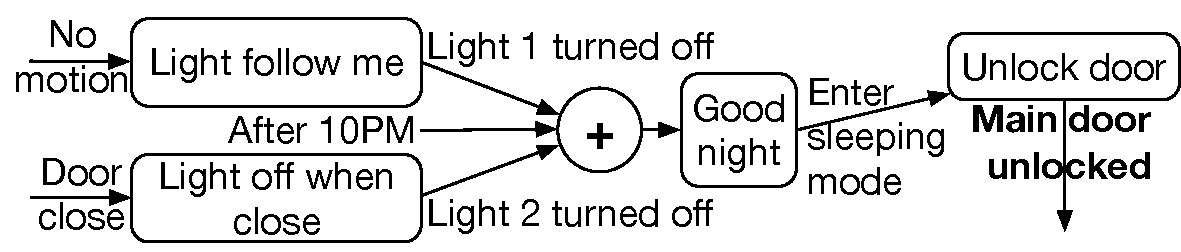
\includegraphics[width=2.8in]{violation_example}
                                \vspace{-0.06in}
                \caption{Example violation due to bad app interactions.}
        \label{violation_example}
    \end{subfigure}\\
    \vspace{0.03in}
    \begin{subfigure}[t]{3.2in}
        \centering
        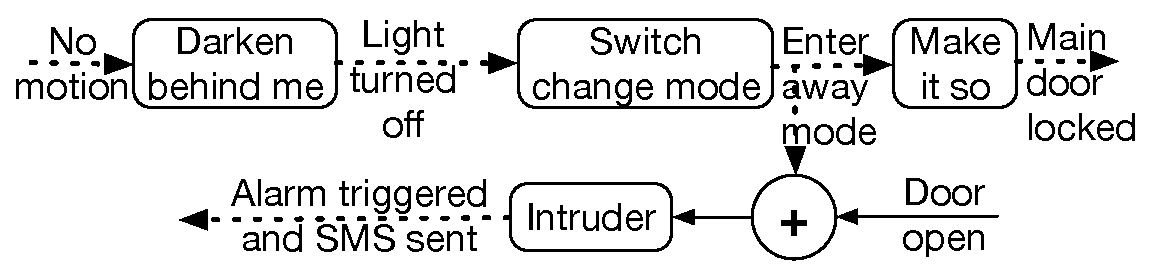
\includegraphics[width=2.8in]{device_failure}
                                \vspace{-0.06in}
        \caption{Example violation due to a device failure. Dotted arrows are
expected events that do not occur due to the failure of the motion sensor.}
                \vspace{-0.1in}
        \label{device_failure}
    \end{subfigure}
    \caption{Violation examples: boxes depict apps and high level abstractions are
shown for inputs/outputs.}
    \label{violationexamples}
\vspace{-0.25in}
\end{figure}
}
\end{comment}


% {\color{black}\sys discovered many serious safety violations, which can be induced by attackers via luring users to install malicious apps (\eg, \texttt{Unlock door} in Figure~\ref{violation_example}) or jamming the report of the motion sensor in Figure~\ref{device_failure}.}
%\vspace{-0.13in}
\section{Violation Attribution}
\sys attributes {\em all} of the ContexIoT's malicious apps~\cite{Jia:contexiot} correctly when each is independently considered
with violation ratios of 100 \% (recall \S\ref{outputanalyzer}). {\color{black}As shown in Table \ref{ContexIoT_apps},}
two apps violated the information leakage property as the command \textit{httpPost} was executed;
two apps violated the ``using security-sensitive command property",
\ie, they generated fake carbon monoxide detection events and an \textit{unsubscribe} is executed;
the remaining 5 apps violated safety properties in the physical space,
\eg, \textit{a main door is unlocked when no one is at home} and, \textit{when smoke is detected, a water valve switch is turned off}.
From among the 11 market apps, 6 were detected with a 100\% violation ratio,
both when verified independently and in conjunction with other apps; they were thus attributed as bad apps.
The remaining were attributed to cause violations (with 70\% or lower violation ratio)
due to bad configurations 
(there existed safe configurations with no violations).

%\vspace{-0.15in}
\section{Scalability}
\begin{comment}
{
\textbf{Runtime}: In all of the experiments we did, the verification halted within a second whenever a violation was present (and
discovered). When no violation was detected, the verification time (of the group from the user study alluded
to before) increases exponentially when the number of generated events increase from 6 to 11, as shown in table \ref{verificationtime}. {\color{black} According to the description in Table \ref{verificationtimesetup} of the devices used in this experiment, we have $(3*2)*(1*2)*(1*5)*(1*3)=180$ options to select a physical event for a sensor at each iteration in Algorithm \ref{alg:smarthingprocess}. If we generate 10 physical events, there are $180^{10}$ permutations of the input sequences. Moreover, each physical event may trigger some new cyber events. This explains the increasing trend of the runtime. Since we ran the experiments in a laptop with limited computing resources, we used 10 events in all of the experiments we did. One may run the experiments with much more generated events in super computing machines or in the cloud to increase the verification coverage. Note that all of the violations we found were detected with just several generated events (\textit{e.g.}, 2 or 3) or even a single event in many cases.}
%\krish{What is the take away here?  It seems abrupt and the reader is left hanging.}
}
\end{comment}

Table~\ref{scalability} shows the scalability benefits of our app dependency analyzer in the above experiments with 150 market apps.
In this table,
``\textit{Original Size}" is the total number of event handlers of a group and
``\textit{New Size}" is the number of event handlers of the largest related set after running the \textit{App Dependency Analyzer} module.
On average, \textit{App Dependency Analyzer} reduced the problem size by a factor 3.4x.


\begin{table}[t]
\ssp
\scriptsize
   %\vspace{-0.13in}
    \caption{Scalability with dependency graphs}
	%\vspace{-0.15in}
    \centering
		%\vspace{-0.05in}
        \label{scalability}
		{
		\begin{tabular}{| c | c | c | c |}
		\hline
		\bf Group & \bf Original Size & \bf New Size & \bf Scale Ratio\\
		\hline
		1 & 37 & 11 & 3.4\\
		\hline
		2 & 27 & 5 & 5.4\\
		\hline
		3 & 34 & 23 & 1.5\\
		\hline
		4 & 30 & 12 & 2.5\\
		\hline
		5 & 42 & 19 & 2.2\\
		\hline
		6 & 34 & 6 & 5.7\\
		\hline
		\multicolumn{3}{|c|}{\textbf{Mean scale ratio}} & \textbf{3.4}\\
		\hline
		\end{tabular}
		}
%\vspace{-0.15in}
\end{table}

\begin{table}[t]
\ssp
\scriptsize
   %\vspace{-0.13in}
    \caption{Runtimes with concurrent and sequential design.}
		%\vspace{-0.05in}
		\centering
        \label{designruntime}
		{
		\begin{tabular}{| c | c | c |}
		\hline
		\bf Number of events & \bf Concurrent & \bf Sequential\\
		\hline
		1 & 1s &  1s\\
		\hline
		2 & 56.5s & 1s\\
		\hline
		3 & 139m & 1s\\
		\hline
		4 & forever &  1s\\
		\hline
		5 &  &  1s\\
		\hline
		6 &  &  4.2s\\
		\hline
		7 &  &  16.3s\\
		\hline
		\end{tabular}
		}
%\vspace{-0.15in}
\end{table}


\begin{table}[tb]
\scriptsize
\ssp
\caption{Verification time vs. number of events.}
%\vspace{-0.1in}
\centering
\label{verificationtime}
{
\begin{tabular}{| c | c | c | c | c | c | c |}
\hline
\bf Number of events & 6 & 7 & 8 & 9 & 10 & 11\\
\hline
\bf Verification time & 6.61s & 50.9s & 396s & 49.83m & 5.89h & 23.39h\\
\hline
\end{tabular}
%\vspace{-0.2in}
}
\end{table}

\begin{comment}
{
\begin{table}[!h]
\scriptsize
\caption{Scalability of dependency graph with market apps.}
\label{scalability}
\centering
\begin{tabular}{| c | c | c | c |}
\hline
Group & Original Size & New Size & Scale Ratio\\
\hline
1 & 37 & 11 & 3.4\\
\hline
2 & 27 & 5 & 5.4\\
\hline
3 & 34 & 23 & 1.5\\
\hline
4 & 30 & 12 & 2.5\\
\hline
5 & 42 & 19 & 2.2\\
\hline
6 & 34 & 6 & 5.7\\
\hline
\multicolumn{3}{|c|}{\textbf{Mean scale ratio}} & \textbf{3.4}\\
\hline
\end{tabular}
\vspace{-0.4in}
\end{table}
}
\end{comment}

%\vspace{-0.13in}
\section{Concurrent vs. Sequential}
%\krish{What two bad groups ? We never said anything here. Can we say, "All bad configurations that were detected, were identified very quickly (within X seconds) by both approaches." Don't think example is needed here.}
%Both of the design approaches detected all of the violations of the two bad groups. Two violations of (Auto Mode Change, Unlock Door) are (i) \textit{a door is unlocked when no one is at home} and (ii) \textit{a door is unlocked when the app is not touched}. One violation of (Brighten Dark Places, Let There Be Dark) is a conflicting command (on \textit{v.s.} off).
Model checkers using both concurrent and sequential design detected all violations
within 1 second. Table~\ref{designruntime} shows the runtimes of the two models with
a good group of apps (\textcolor{black}{2 apps and 7 devices}), which does not violate any property.
We see that sequential design significantly reduces the runtime of the verification.
Note that \textit{forever} means the experiment ran for a week and then was forced to stop.
Moreover, we also verified the runtime of our sequential approach with a much bigger system,
which comprises of 5 related apps and 10 devices and does not have any violation.
{\color{black}As shown in Table~\ref{verificationtime}}, the verification time for 10 events is about 5 hours,
which is quite reasonable for a laptop with limited computing resources.
%We point out that in all of the experiments we did, the violations were detected within {\color{black}several seconds}.
%Recall that as demonstrated in our volunteer experiments,
%humans cannot easily detect unintended bad consequences of complex app interactions
%even given time.